\chapter{Methods}\label{ch2:methods}

\section{Approach}\label{sec1:approach} 

\section{Hypotheses}

 hypotheses of this thesis are as follows:
1) Te MPI 2020 paper, which produces good disparity maps for <the opposite of close-up shots> <long shots of objects/landscapes> \cite{}, is unable to do so for close-up shot of people/objects. When we re-recreated the 202 Hence, our first hypothesis is that re-retraining the re-created 2020 MPI model on  


xxxxxxxxxxxxxxxxxxxxxxxxxxxxxxxxxxxxxxxxxxxxxxxxxx

Stereo Magnification (2018) paper introduces the MPI representation and also explains how the data was processed. Some parts of the code are refactored and reused in the 2020 MPI paper like how the 2018 paper loads data in: in particular the data loader (loader.py, datasets.py) does subsequence selection and some slight random cropping. There are several more interesting MPI-related papers (Pushing the Boundaries, DeepView, Local Lightfield Fusion) which explore different directions, but none of them are tackling the single-view approach.

richard tucker email very very important:

In terms of relation to the previous MPI papers: Stereo Magnification (2018) introduces the representation and also explains how the data was processed. The code itself is separate but you could look at how it loads data in: in particular the data loader (loader.py, datasets.py) does subsequence selection and some slight random cropping.

From the code we have released (https://github.com/google-research/google-research/tree/master/single_view_mpi) you can see:
  • our the network definition (convolutional layers, kernel sizes, etc) (nets.mpi_from_image)
  • how to render views from new camera positions (mpi.render), including all the homography stuff

What you don't have is (a) the implementation of the losses, and (b) data including point clouds and a way to load it in.
One of the key points of Single-View View Synthesis was to use sparse point cloud data to make the view synthesis loss scale-invariant. To obtain such data you would have to process the mannequin dataset to obtain point cloud and/or depth, for example with COLMAP (maybe you have already done that), and then you could write a data loader or extend the one from Stereo Magnification.

Is your Mannequin Dataset this one: https://google.github.io/mannequinchallenge/www/index.html? If so, a note of caution: it's quite a bit smaller than RealEstate10K, and so there is a risk of overfitting. (I have tried training on something like it myself, and I found that it was better to use a combination of both RealEstate and MannequinChallenge than just MannequinChallenge alone). But anyway, that's something to worry about after you are able to train.

xxxxxxxxxxxxxxxxxxxxxxxxxxxxxxxxxxxxxxxxxxxxxxxxxxxxxxx

Whereas the 2018 model claioms to gebreraLIZER TO OTHER DATASEYT WIERHOUT RETREAINGU, no suvk ckaimsd gave been madfe by the 2020 model

When we ran the inference part of the 2020 Single-View MPI model \footnote{Deep Learning terms such as model, network, and CNN have been used interchangeably throughout this thesis.} on a video chat frame and found that the generated disparity map (a by-product of MPI inference in this network architecture) was visually inaccurate, it became the starting off point for our thesis. Comparatively, the inferred disparity map would be much more visually accurate when a real estate video frame was processed. The latter outcome is to be expected because the 2020 Single-View MPI model was exclusively trained on the RealEstate10K video dataset.   

\subsection{Problem Statement 1}\label{subsec1:problem_statement_1}

\textbf{How to increase the 2020 Single-View MPI model’s depth prediction accuracy for video chat frames or any other video-chat-relevant image with close up shots of people.}

As inference was one of the only parts of the network made publicly available by the authors on GitHub due to the proprietary nature of some other aspects of their code, the first step in addressing problem statement 1 was to recreate the 2020 Single-View MPI training procedure.

Recreating and retraining the network involved the following:
\begin{itemize}
    \item Taking the readily available network information from the paper --- like details about the various types of fully-convolutional encoder-decoder layers involved, etc. --- and putting it in place with other aspects of the network that called for a more involved recreation process like the data loader part and the loss function.
    \item Processing all the videos from the required datasets with an ORB-SLAM2 package called COLMAP to extract the 3D point clouds of the scenes in each video frame which makes up one-half of the input to the training pipeline, the other half being the actual video frames themselves.
    \item Attempting to train the network on only the video-chat-relevant Mannequin Challenge video dataset \cite{li2019learning} which is $\sim$90\% smaller than the RealEstate10K dataset.
    \item Fixing the programming errors encountered during training.
    \item Retraining the recreated model on not just the Mannequin Challenge dataset but also the RealEstate10K dataset by clubbing both datasets together to be used as a singular source of input to the recreated 2020 MPI model.
\end{itemize}

The main reason for extending the Mannequin Challenge dataset with the originally used RealEstate10K dataset was so Hypothesis B of this thesis could be proved: ---

\paragraph{Hypothesis A:}
The recreated model trained only on the video-chat-relevant Mannequin Challenge Dataset performs as well as the 2020 MPI model does on real estate data, when it comes to accurately predicting MPIs and disparity maps of video-chat-relevant frames involving close up shots of one or more persons.

\paragraph{Hypothesis B:}
If hypothesis A is disproved\footnote{Please refer to the Experiments and Results Chapter.}, the recreated MPI model should perform as well as the 2020 MPI model if the Mannequin Challenge training data were extended by the RealEstate10K dataset.

\section{Data}\label{sec:data} 

Both Mannequin Challenge~\cite{li2019learning} and RealEstate10K~\cite{zhou2018stereo} datasets were created by roughly the same group of researchers hailing from Google. They involved the same ORB-SLAM2, COLMAP, and scale-normalization procedures of Zhou et al.~\cite{zhou2018stereo} (Subsection~\ref{subsec:base-papers}). Hence, both datasets consist of the same kind of metadata in text files pertaining to the downloadable videos. Each text file begins with the video’s YouTube link on the first line and continues with the details of each COLMAP-processed video frame from the second line onward. Frame details include the timestamp (in microseconds), camera intrinsics, and camera extrinsics. As mentioned in subsection~\ref{subsec:base-papers}, COLMAP is a 3D scene reconstruction pipeline. It attempts to recover the 3D scene structure from even those unstructured 2D images of the scene that do not come tagged with any prior knowledge of camera intrinsics, extrinsics, and nature of objects captured. The extracted scene structure is either in the form of sparse 3D points along with the camera parameters for each input 2D image or in the form of dense 3D points with associated color information. COLMAP's pipeline can be given by: feature detection $\rightarrow$ pairwise feature matching  $\rightarrow$ correspondence estimation $\rightarrow$ incremental structure from motion (Figure~\ref{fig:colmap-photogrammetry-pipeline}). Fortunately, absolute camera poses are not required by the model; only the relative ones made available with the help of COLMAP in these text files are. Our scripts to download and curate all these videos were facilitated by our compilation of a comprehensive Docker container ensuring robustness in code reusability and transferability. Resolving version compatibility issues among our project dependencies such as COLMAP and OpenFace 2.2, both in the Docker container and in Google Colaboratory proved paramount to the successful running of our experiments. All our scripts, notebooks, sample renderings, demos, and most other aspects of our code for this project can be found in our GitHub repository (Section~\ref{sec:code-sources}).

\begin{figure}[!h]
    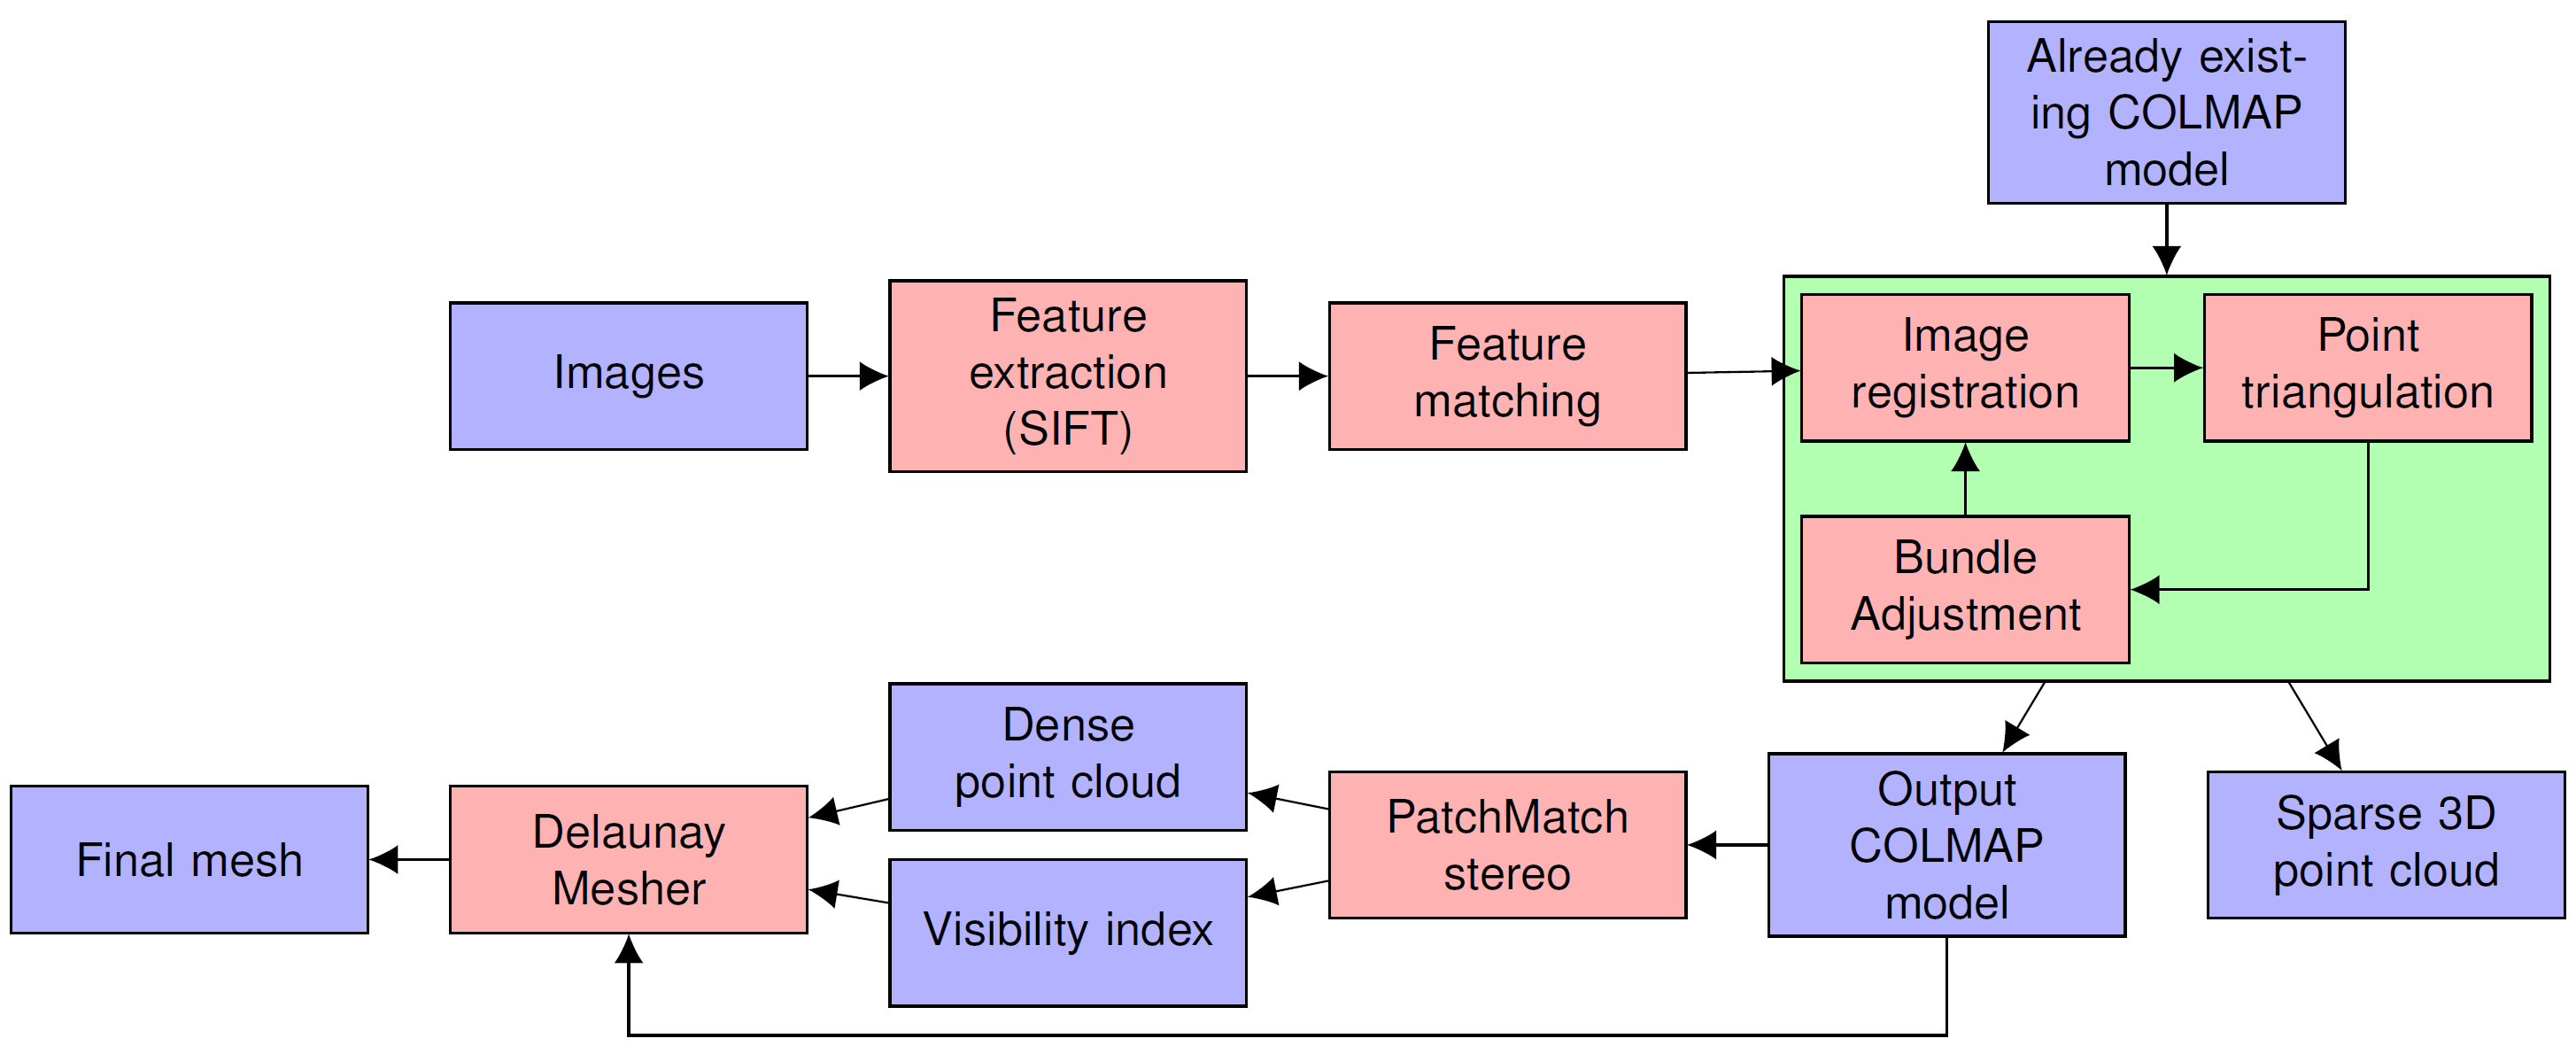
\includegraphics[width=1\columnwidth]{figures/colmap-photogrammetry-pipeline.png}
    \caption{Photogrammetry workflow used in COLMAP~\cite{pinard_does_2021}}
    \label{fig:colmap-photogrammetry-pipeline}
\end{figure}
    
Although our training and testing scripts are designed to crop all incoming video frames to 512$\times$512 pixels, we ensured that we downloaded all videos with youtube-dl at 720p resolution. This uniformity was so we could reduce the number of sources of arbitrariness in the initial process of replicating Tucker and Snavely's~\cite{single_view_mpi} work. Linking youtube-dl with the download management utility aria2~\cite{noauthor_aria2_2021} proved very useful in bolstering youtube-dl’s download speed by optimizing resource utilization. We then targeted addressing youtube-dl download errors. There would inevitably be several partial and/or skipped downloads for various reasons ranging from the videos being taken down from YouTube over time to fixable errors intrinsic to youtube-dl. Moreover, some videos were unavailable in their 720p versions and were discarded by us with the aim of maintaining consistency. In favor of maintaining the pristine versions we chose not to manually convert the varying resolutions to 720p. Although differently scaled videos should theoretically not pose any problem to training or to 3D point cloud generation with COLMAP, we opted again to go with uniformity and consequent ease of reproducibility for one and all.
    
We were finally able to procure 66,861 RealEstate10K videos with 9,095,528 frames and 2,364 MannequinChallenge videos with 117,811 frames, for processing. But not all downloaded videos could be processed. For instance, only $\sim$60000 RealEstate10K videos were actually COLMAP-processed and used for training. This is because the rest of the videos did not meet COLMAP processing requirements. And, it would have taken 200 days to process all 66,861 videos with COLMAP with CPUs alone. Fortunately, we were able to avail the benefits NVIDIA Tesla V100 GPUs (rated the best server models in 2020) at Cal Poly and could bring down the processing time to 25 days. In these ways, we obtained the required points clouds and frames for both training and testing.
















\section{Implementation}\label{sec:implementation} 

We attempted to generate accurate MPI representations for close-up targets such as heads and upper bodies, and improve the pixel accuracies of views synthesized from these MPIs. After putting together the data loader to feed the datasets and point clouds into the network, we recreated loss functions from the textual descriptions in the single-view MPI paper. As mentioned in subsection~\ref{subsec:base-papers}, we likened our training process to Tucker and Snavely~\cite{single_view_mpi} with regard to various aspects such as the use of TensorFlow 2.2, ADAM solver, a pixel loss weight of 1, a smoothness loss weight of 0.5, etc. We experimented with choices of learning rate and depth loss weight but generally picked 0.00001 and 1, respectively, contrary to the 0.0001 and 0.1 used in Tucker and Snavely. We reduced the learning rate because we were fine-tuning the pretrained model rather than training from scratch. The requirement that we had to have view synthesis quality as supervision was fulfilled by taking a frame one frame apart from each chosen training frame as target ground truth. We trained for a number of steps rather than for a number of epochs. Our data loader randomizes batch picking not only for testing but also for training. Moreover, we have not yet been able to go beyond the model experimentation stage. Exposing the model to a wide variety of frames is the way to go in this stage. For the model to be training sequentially on all frames clip by clip, and covering entire datasets multiple times in multiple epochs, it should be free of any errors that impede its progress toward convergence. We have not been able to bring our model up to that stage yet. 

We used wandb.ai~\cite{wandb} for experiment tracking and it proved to be a valuable tool for our entire process. It helped us spin different variants of the model, chiefly characterized by their being trained either on MannequinChallenge alone or on a combination of both datasets. As with some notable attempts at model training in the community, we encountered Not a Number (NaN) gradient errors that took a good chunk of our resolution efforts in this work, but ultimately could not be resolved. NaN losses signal that the issue of vanishing/exploding gradients may be present. In this work, NaN gradients could only be reduced in their frequency of occurrence from once in several hundred steps to once in several thousand steps. wandb.ai helped immensely in resuming not just the training runs themselves but also the activity of logging training metrics right from the point where the run broke off due to a NaN error. What also helped bring down the frequency of encountering NaNs, we believe, was the fact that we removed all those videos from the training/testing process that had at least one frame with a point cloud composed of less than two 3D points. Our Linux command to locate such point cloud \texttt{.txt} files (Section~\ref{sec:code-snippets}) would take about 3 hours to sift through a set of 2500 point cloud directories with one \texttt{.txt} file per video frame. Replacing \texttt{cumprod} used in several places in the single-view MPI source code with \texttt{safe\_cumprod}, as suggested to us by one of the authors of the single-view paper, also helped reduce the frequency of encountering NaNs. One of the issues that we were able to completely resolve was the occasional throwing of \texttt{ValueErrors} by our data loader. We also attempted to redress the rendered artifacts mentioned in section~\ref{sec:approach} and determine if real-time, high-quality view synthesis was indeed possible without game engines.

We used customized training loops with TensorFlow's \texttt{tf.GradientTape} context~\cite{noauthor_custom_nodate}. However, we found that the gradient calculation (Section~\ref{sec:code-snippets}) would take about one minute! We were using a batch size of 8 at that time on an NVIDIA V100 GPU. But the authors of the single-view MPI paper informed us that their gradient calculation would take less than a second even on a single worker. They then correctly diagnosed our issue to be that we were doing everything in \textit{eager mode}, which would lead to the accumulation of a lot of overhead. They suggested that using Keras's \texttt{model.fit}, or using the old estimator system of TensorFlow, or just wrapping things in \texttt{tf.function} should allow the critical parts to run in graph mode and be faster. They also suggested that things were probably too big to fit on our GPU. The authors had used a batch size of 4. We ultimately adopted the use of \texttt{tf.function} wrapper as well as a batch size of 4 and were able to complete implementing our training and testing pipelines.

\begin{figure}[!h]
    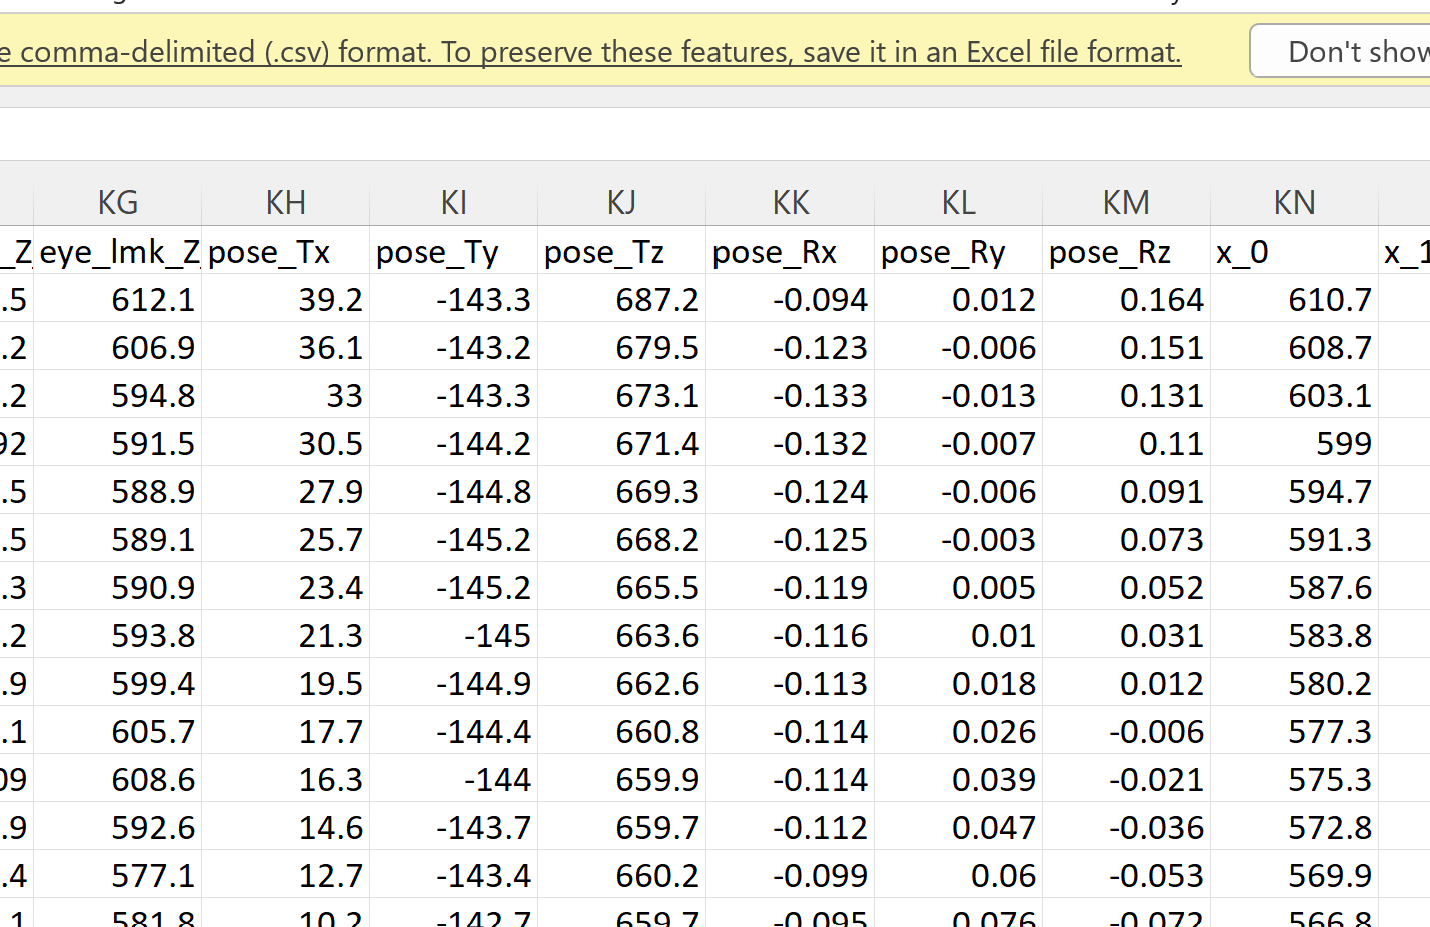
\includegraphics[width=0.75\columnwidth]{figures/openface-csv.png}
    \caption{A Snapshot of OpenFace 2.2~\cite{baltrusaitis_openface_2018} Outputs}
    \label{fig:openface-outputs}
\end{figure}

We then inserted OpenFace 2.2~\cite{baltrusaitis_openface_2018} into the inference pipeline of one of our better performing model variants and attempted to emulate a video chat system, one half at a time. We subjected a ``viewer" video sequence to head pose extraction by OpenFace 2.2 from all frames, as show in figure~\ref{fig:3d-video-chat-rendering-pipeline}. We used one of the utility functions in the single-view MPI modules to extract the yaw, pitch, and roll angles of the ``viewer" frames in a manner conducive to being accepted by the MPI inference. We then rendered the ``viewee" video sequence at the head pose of the ``viewer" frames with matching timestamps. Perhaps more precision could have been added by using not just head pose estimation but also gaze estimation with OpenFace. A snapshot of OpenFace 2.2 outputs for multiple frames in a sequence is shown in figure~\ref{fig:openface-outputs}

